\documentclass[
	a4paper,
	oneside,
	BCOR = 10mm,
	DIV = 12,
	12pt,
	headings = normal,
]{scrartcl}

%%% Length calculations
\usepackage{calc}
%%%

%%% Support for color
\usepackage{xcolor}
\definecolor{lightblue}{HTML}{03A9F4}
\definecolor{red}{HTML}{F44336}
%%%

%%% Including graphics
\usepackage{graphicx}
%%%

%%% Font selection
\usepackage{fontspec}

\setromanfont{STIX Two Text}[
	SmallCapsFeatures = {LetterSpace = 8},
]

\setsansfont{IBM Plex Sans}[
	Scale = MatchUppercase,
]

\setmonofont{IBM Plex Mono}[
	Scale = MatchUppercase,
]
%%%

%%% Math typesetting
\usepackage{amsmath}

\usepackage{unicode-math}
\setmathfont{STIX Two Math}

\usepackage{IEEEtrantools}
%%%

%%% List settings
\usepackage{enumitem}
\setlist[enumerate]{
	label*      = {\arabic*.},
	left        = \parindent,
	topsep      = 0\baselineskip,
	parsep      = 0\baselineskip,
	noitemsep, % override itemsep
}
% List settings for levels 2–4
\setlist[enumerate, 2, 3, 4]{
	label*      = {\arabic*.},
	left        = 0em,
	topsep      = 0\baselineskip,
	parsep      = 0\baselineskip,
	noitemsep, % override itemsep
}

\setlist[itemize]{
	label*      = {—},
	left        = \parindent,
	topsep      = 0\baselineskip,
	parsep      = 0\baselineskip,
	itemsep     = 1\baselineskip,
	noitemsep, % override itemsep
}

\setlist[description]{
	font        = {\rmfamily\upshape\bfseries},
	topsep      = 1\baselineskip,
	parsep      = 0\baselineskip,
	itemsep     = 0\baselineskip,
}

%%%

%%% Structural elements typesetting
\setkomafont{pagenumber}{\rmfamily\upshape}
\setkomafont{disposition}{\rmfamily\bfseries}

% Sectioning
\RedeclareSectionCommand[
	beforeskip = -1\baselineskip,
	afterskip  = 1\baselineskip,
	font       = {\normalsize\bfseries\scshape},
]{section}

\RedeclareSectionCommand[
	beforeskip = -1\baselineskip,
	afterskip  = 1\baselineskip,
	font       = {\normalsize\bfseries\itshape},
]{subsection}

\RedeclareSectionCommand[
	beforeskip = -1\baselineskip,
	afterskip  = 1\baselineskip,
	font       = {\normalsize\bfseries},
]{subsubsection}

\RedeclareSectionCommand[
	beforeskip = -1\baselineskip,
	afterskip  = -0.5em,
	font       = {\normalsize\mdseries\scshape\addfontfeatures{Letters = {UppercaseSmallCaps}}},
]{paragraph}
%%%

%%% Typographic enhancements
\usepackage{microtype}
%%%

%%% Language-specific settings
\usepackage{polyglossia}
\setmainlanguage{ukrainian}
\setotherlanguages{english}
%%%

%%% Captions
\usepackage{caption}
\usepackage{subcaption}

%\DeclareCaptionLabelFormat{closing}{#2)}
%\captionsetup[subtable]{labelformat = closing}

%\captionsetup[subfigure]{labelformat = closing}

\captionsetup[table]{
	aboveskip = 0\baselineskip,
	belowskip = 0\baselineskip,
}

\captionsetup[figure]{
	aboveskip = 1\baselineskip,
	belowskip = 0\baselineskip,
}

\captionsetup[subfigure]{
	labelformat = simple,
	labelformat = brace,
	justification = RaggedRight,
	singlelinecheck = false,
}
%%%

%%% Hyphenated ragged typesetting
\usepackage{ragged2e}
%%%

%%% Table typesetting
\usepackage{booktabs}
\usepackage{longtable}

\usepackage{multirow}

\usepackage{array}
\newcolumntype{v}[1]{>{\RaggedRight\arraybackslash\hspace{0pt}}p{#1}}
\newcolumntype{b}[1]{>{\Centering\arraybackslash\hspace{0pt}}p{#1}}
\newcolumntype{n}[1]{>{\RaggedLeft\arraybackslash\hspace{0pt}}p{#1}}
%%%

%%% Drawing
\usepackage{tikz}
\usepackage{tikzscale}
\usetikzlibrary{positioning}
\usetikzlibrary{arrows.meta} % Stealth arrow tips
%%%

%%% SI units typesetting
\usepackage{siunitx}
\sisetup{
	output-decimal-marker = {,},
	exponent-product      = {\cdot},
	inter-unit-product    = \ensuremath{{} \cdot {}},
	per-mode              = symbol,
}
%%%

% Code Highlighting
\usepackage{minted}
\setmintedinline{
	style = bw,
	breaklines,
}

\newminted[bashterm]{text}{%
	autogobble,%
	breaklines,%
	style=bw,%
}

\newminted[codegeneric]{text}{%
	autogobble,%
	style=bw,%
	breaklines,%
	fontsize=\small,%
}

\newmintinline{bash}{%
}

\newmintinline[minttext]{text}{%
	breaklines,%
	breakanywhere,%
}

%%% Framing code listings
\usepackage{tcolorbox}
\tcbuselibrary{breakable}
\tcbuselibrary{minted}
\tcbuselibrary{skins}

% Text file listing
\newtcblisting[
	auto counter,
	list inside,
	number within = section,
]{listingplaintext}[3][]{%
	minted language = text,
	minted style    = bw,
	minted options  = {
		autogobble,
		linenos,
		tabsize = 4,
		breaklines,
		breakanywhere,
		fontsize = \footnotesize,
	},
	empty,
	sharp corners,
	coltitle = black,
	borderline horizontal = {1pt}{0pt}{black},
	titlerule = {0.5pt},
	titlerule style = {
		black,
	},
	toptitle = 0.3em,
	bottomtitle = 0.3em,
	before skip      = \intextsep,
	after  skip      = \intextsep,
	title            = {Лістинг \thetcbcounter: #2},
	list entry       = {\protect\numberline{\thetcbcounter}#2},
	left = 0em,
	right = 0em,
	%
	listing only,
	breakable,
	%
	label = {#3},%
}

\newtcbinputlisting[
	use counter from = listingplaintext,
	list inside,
	number within = section
]{\inputplaintext}[4][]{%
	minted language = text,
	minted style    = bw,
	minted options  = {
		autogobble,
		linenos,
		tabsize = 4,
		breaklines,
		breakanywhere,
		fontsize = \footnotesize,
	},
	empty,
	sharp corners,
	coltitle = black,
	borderline horizontal = {1pt}{0pt}{black},
	titlerule = {0.5pt},
	titlerule style = {
		black,
	},
	toptitle = 0.3em,
	bottomtitle = 0.3em,
	before skip      = \intextsep,
	after  skip      = \intextsep,
	title            = {Лістинг \thetcbcounter: #3},
	list entry       = {\protect\numberline{\thetcbcounter}#3},
	left = 0em,
	right = 0em,
	%
	listing file={#2},
	listing only,
	breakable,
	%
	label = {#4}
}

\newtcblisting[
	use counter from = listingplaintext,
	list inside,
	number within = section,
]{listingpython}[3][]{%
	minted language = python,
	minted style    = bw,
	minted options  = {
		autogobble,
		linenos,
		tabsize = 4,
		breaklines,
		breakanywhere,
		fontsize = \footnotesize,
	},
	empty,
	sharp corners,
	coltitle = black,
	borderline horizontal = {1pt}{0pt}{black},
	titlerule = {0.5pt},
	titlerule style = {
		black,
	},
	toptitle = 0.3em,
	bottomtitle = 0.3em,
	before skip      = \intextsep,
	after  skip      = \intextsep,
	title            = {Лістинг \thetcbcounter: #2},
	list entry       = {\protect\numberline{\thetcbcounter}#2},
	left = 0em,
	right = 0em,
	%
	listing only,
	breakable,
	%
	label = {#3},
	%
	#1%
}

\newtcbinputlisting[
	use counter from = listingplaintext,
	list inside,
	number within = section
]{\inputpython}[4][]{%
	minted language = python,
	minted style    = bw,
	minted options  = {
		autogobble,
		linenos,
		tabsize = 4,
		breaklines,
		breakanywhere,
		fontsize = \footnotesize,
	},
	empty,
	sharp corners,
	coltitle = black,
	borderline horizontal = {1pt}{0pt}{black},
	titlerule = {0.5pt},
	titlerule style = {
		black,
	},
	toptitle = 0.3em,
	bottomtitle = 0.3em,
	before skip      = \intextsep,
	after  skip      = \intextsep,
	title            = {Лістинг \thetcbcounter: #3},
	list entry       = {\protect\numberline{\thetcbcounter}#3},
	left = 0em,
	right = 0em,
	%
	listing file={#2},
	listing only,
	breakable,
	%
	label = {#4}
}

% Linux command-line listing
\newtcblisting{linuxterm}%
{%
	% Syntax highlighing options
	listing only,%
	minted language = bash,%
	minted options={%
		autogobble,%
		linenos%
	},%
	% Presentation options
	empty,%
	%% Margins
	sharp corners,%
	toptitle = 0.0em,%
	bottomtitle = 0.0em,%
	left = 0em,%
	right = 0em,%
	before skip = \intextsep,%
	after skip = \intextsep,%
}

\newtcblisting{linuxtermout}%
{%
	% Syntax highlighing options
	listing only,%
	minted language = text,%
	minted options={%
		autogobble,%
		linenos%
	},%
	% Presentation options
	empty,%
	%% Margins
	sharp corners,%
	toptitle = 0.0em,%
	bottomtitle = 0.0em,%
	left = 0em,%
	right = 0em,%
	before skip = \intextsep,%
	after skip = \intextsep,%
}

% Dockerfile listings
\newtcblisting[
	use counter from = listingplaintext,
	list inside,
	number within = section,
]{listingdocker}[3][]{%
	minted language = dockerfile,
	minted style    = bw,
	minted options  = {
		autogobble,%
		linenos,
		tabsize = 4,
		breaklines,
		breakanywhere,
		fontsize = \footnotesize,
	},
	empty,
	sharp corners,
	coltitle = black,
	borderline horizontal = {1pt}{0pt}{black},
	titlerule = {0.5pt},
	titlerule style = {
		black,
	},
	toptitle = 0.3em,
	bottomtitle = 0.3em,
	before skip      = \intextsep,
	after  skip      = \intextsep,
	title            = {Лістинг \thetcbcounter: #2},
	list entry       = {\protect\numberline{\thetcbcounter}#2},
	left = 0em,
	right = 0em,
	%
	listing only,
	breakable,
	%
	label = {#3},%
}

% Docker Compose listings
\newtcblisting[
	use counter from = listingplaintext,
	list inside,
	number within = section,
]{listingdockercompose}[3][]{%
	minted language = yaml,
	minted style    = bw,
	minted options  = {
		autogobble,%
		linenos,
		tabsize = 4,
		breaklines,
		breakanywhere,
		fontsize = \footnotesize,
	},
	empty,
	sharp corners,
	coltitle = black,
	borderline horizontal = {1pt}{0pt}{black},
	titlerule = {0.5pt},
	titlerule style = {
		black,
	},
	toptitle = 0.3em,
	bottomtitle = 0.3em,
	before skip      = \intextsep,
	after  skip      = \intextsep,
	title            = {Лістинг \thetcbcounter: #2},
	list entry       = {\protect\numberline{\thetcbcounter}#2},
	left = 0em,
	right = 0em,
	%
	listing only,
	breakable,
	%
	label = {#3},%
}


% Customize minted line numbers
\renewcommand{\theFancyVerbLine}{\ttfamily\scriptsize\arabic{FancyVerbLine}}

%%%

%%% Typeset menus and keys
\usepackage{menukeys}[
	os=win,
]
%%%

%%% Links and hyperreferences
\usepackage{hyperref}
\hypersetup{
	bookmarksnumbered = true,
	colorlinks      = false,
	linkbordercolor = red,
	urlbordercolor  = lightblue,
	pdfborderstyle  = {/S/U/W 1.5},
}
%%%

%%% Length adjustment

% Set baselineskip, default is 14.5 pt
\linespread{1.068966} % ~15.5 pt
\setlength{\emergencystretch}{1em}
\setlength{\parindent}{1.5em}
\newlength{\gridunitwidth}
\setlength{\gridunitwidth}{\textwidth / 12}
%%%

%%% Custom commands
\newcommand{\allcaps}[1]{%
	{%
		\addfontfeatures{%
			Letters = UppercaseSmallCaps,
			LetterSpace = 8,%
		}%
		#1%
	}%
}
\newcommand{\filename}[1]{\texttt{#1}}
\newcommand{\progname}[1]{\texttt{#1}}
\newcommand{\commandname}[1]{\texttt{#1}}
\newcommand{\modulename}[1]{\texttt{#1}}
\newcommand{\ifname}[1]{\texttt{#1}} % typesets a network interface's name

\newcommand{\transeng}[1]{{англ.}~\textit{\textenglish{#1}}}
%%%

%%% Custom math commands
\newcommand{\longvar}[1]{\mathit{#1}}
%%%

\begin{document}

\begin{titlepage}
		\begin{center}
			Міністерство освіти і~науки України\\
			Національний авіаційний університет\\
			Факультет кібербезпеки, комп'ютерної та~програмної інженерії\\
			Кафедра комп'ютеризованих систем управління

			\vspace{\fill}
				Лабораторна робота №~2.4\\
				з~дисципліни «Захист інформації в~комп'ютерних системах»\\
				на~тему «Криптографічні програмні засоби з відкритим ключем»

			\vspace{\fill}

			\begin{flushright}
				Виконав:\\
				студент \allcaps{ФККПІ}\\
				групи \allcaps{СП}-425\\
				Клокун В.\,Д.\\
				Перевірила:\\
				Супрун О.\,М.
			\end{flushright}

			Київ 2019
		\end{center}
	\end{titlepage}

	\section{Мета роботи}
		Ознайомитися з~основними поняттями асиметричних криптографічних систем.

	\section{Завдання роботи}
		Встановити програмне забезпечення для ОС Windows та GNU/Linux, що виконує криптографічні операції з відкритим ключем, та навчитися його використовувати.

	\section{Хід~роботи}
		\subsection{Асиметричне шифрування в операційній системі~\textenglish{Windows}}
			Щоб виконати лабораторну роботу, готуємо систему під управлінням операційної системи~\textenglish{Windows} і встановлюємо на неї програмний продукт~\textenglish{\allcaps{PGP} Desktop}. Встановивши його, генеруємо публічний та приватний ключі для асиметричного шифрування~(рис.~\ref{fig:pk-generation}).

		\begin{figure}[!htbp]
			\begin{subfigure}[b]{6 \gridunitwidth - 1em / (2-1)}
				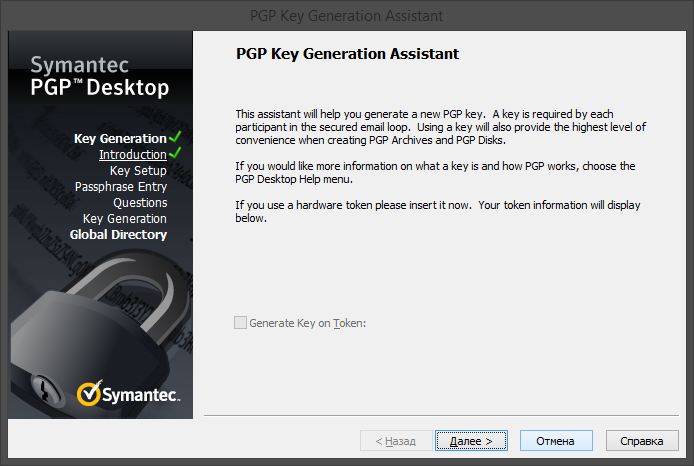
\includegraphics[width = \columnwidth]{./assets/p01.png}
				\caption{}
				\label{subfig:pk-assistant-start}
			\end{subfigure}%
			\hspace{1em}%
			\begin{subfigure}[b]{6 \gridunitwidth - 1em / (2-1)}
				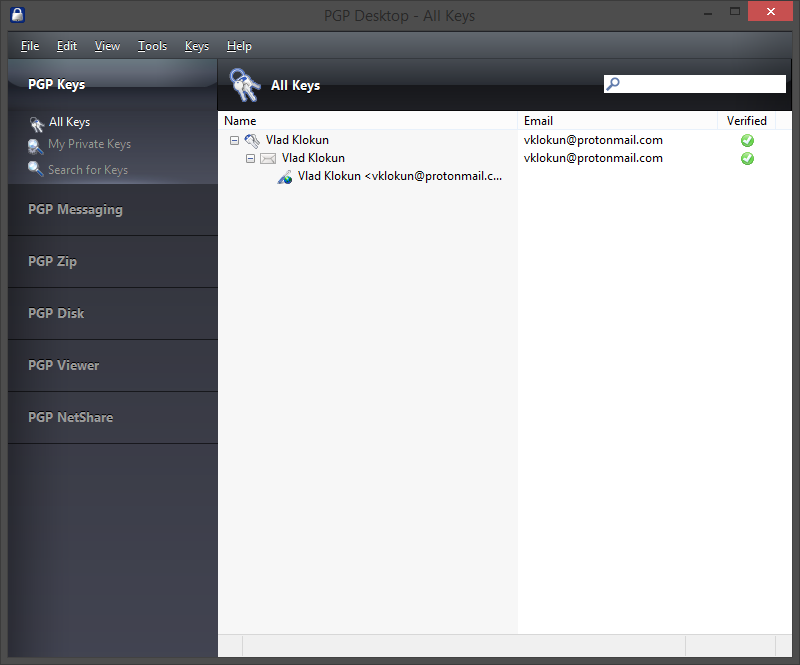
\includegraphics[width = \columnwidth]{./assets/p06.png}
				\caption{}
				\label{subfig:pk-assistant-res}
			\end{subfigure}
			\caption{Створення пари ключів: публічного і приватного}
			\label{fig:pk-generation}
		\end{figure}

		Експортуємо створений публічний ключ~(рис.~\ref{fig:pk-export}). Для цього обираємо створений ключ, викликаємо контекстне меню, обираємо пункт \menu{Export...} і зберігаємо у бажаній директорії.

		\begin{figure}[!htbp]
			\centering
			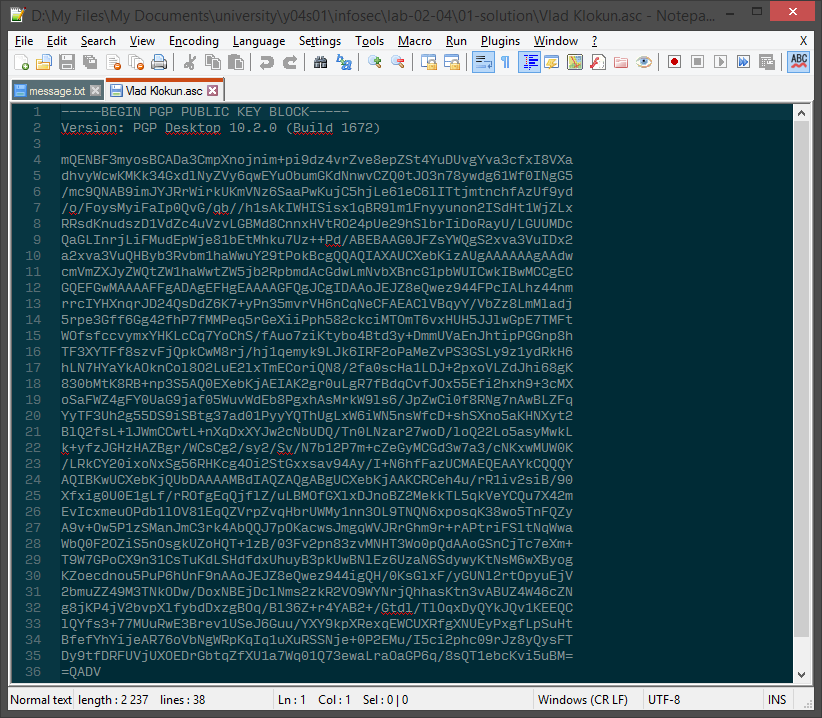
\includegraphics[width = 6\gridunitwidth]{./assets/p06-02.png}
			\caption{Результат експорту створеного публічного ключа}
			\label{fig:pk-export}
		\end{figure}

		Переглядаємо список ключів, до яких має доступ наша криптографічна система з відкритим ключем~\allcaps{(КСВК)}~(рис.~\ref{fig:pks-available}).

		\begin{figure}[!htbp]
			\centering
			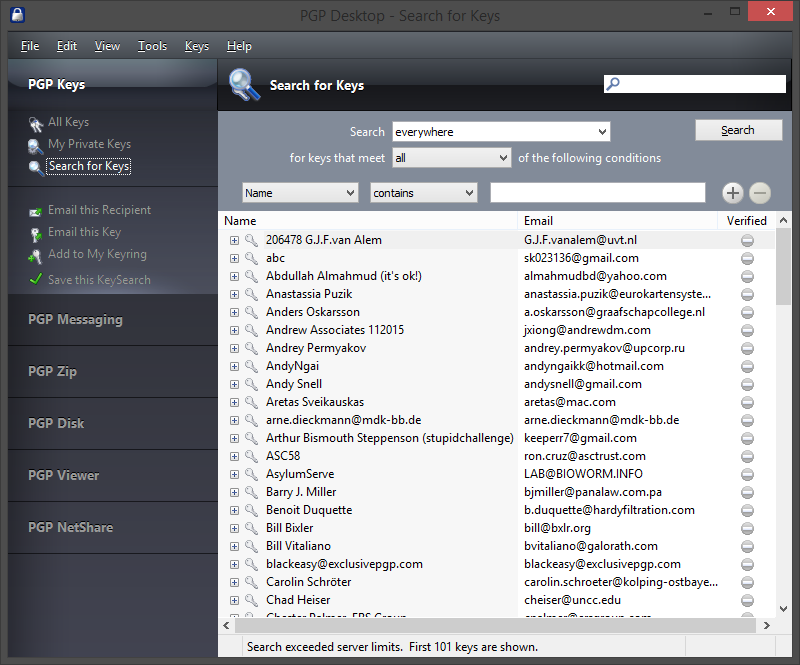
\includegraphics[width = 6\gridunitwidth]{./assets/p07.png}
			\caption{Список ключів, доступних системі}
			\label{fig:pks-available}
		\end{figure}

		Знаходимо відкриті ключі інших осіб та завантажуємо будь який з них, а також перевіряємо його цілісність за наведеним відбитком і імпортуємо його~(рис.~\ref{fig:pk-import}).

		\begin{figure}[!htbp]
			\centering
			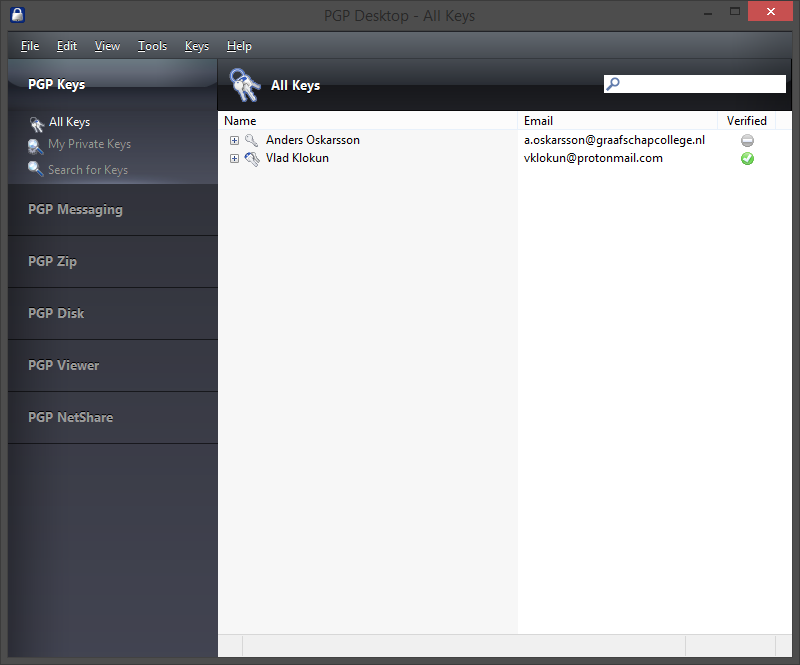
\includegraphics[width = 6\gridunitwidth]{./assets/p08.png}
			\caption{Результат імпорту ключа}
			\label{fig:pk-import}
		\end{figure}

		Шифруємо просте повідомлення за допомогою власного публічного ключа. Отримавши результат шифрування, розшифровуємо його і перевіряємо дані~(рис.~\ref{fig:enc-dec-file}).

		\begin{figure}[!htbp]
			\begin{subfigure}[b]{8 \gridunitwidth - 1em / (2-1)}
				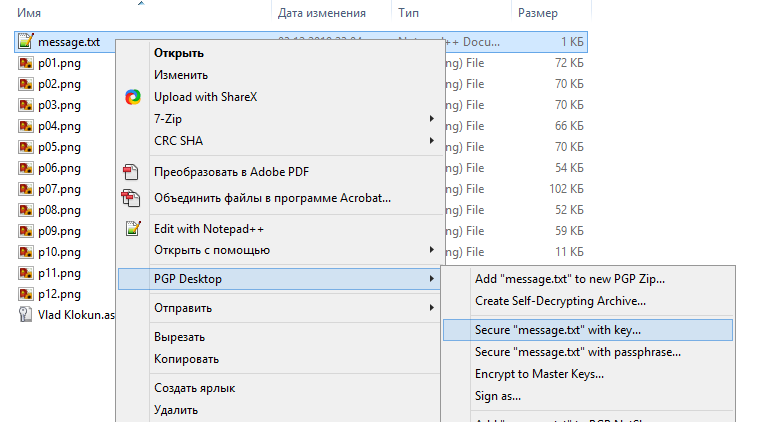
\includegraphics[width = \columnwidth]{./assets/p13.png}
				\caption{}
				\label{subfig:enc}
			\end{subfigure}%
			\hspace{1em}%
			\begin{subfigure}[b]{4 \gridunitwidth - 1em / (2-1)}
				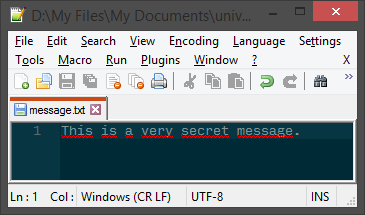
\includegraphics[width = \columnwidth]{./assets/p15.png}
				\caption{}
				\label{subfig:dec}
			\end{subfigure}
			\begin{subfigure}[b]{8 \gridunitwidth - 1em / (2-1)}
				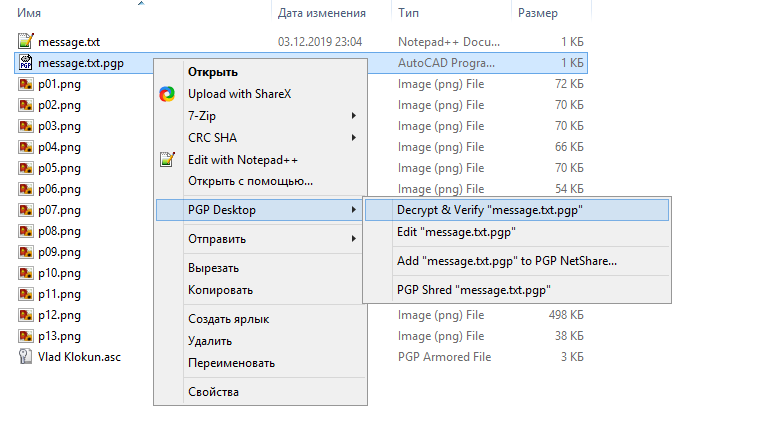
\includegraphics[width = \columnwidth]{./assets/p14.png}
				\caption{}
				\label{subfig:dec}
			\end{subfigure}
			\caption{Шифрування, розшифрування і результат}
			\label{fig:enc-dec-file}
		\end{figure}

		Підписуємо файл цифровим підписом та передаємо файл і цифровий підпис товаришу. Отримуємо аналогічну пару від товариша і перевіряємо справжність файлу~(рис.~\ref{fig:sign-verify-file}).

		\begin{figure}[!htbp]
			\begin{subfigure}[b]{6 \gridunitwidth - 1em / (2-1)}
				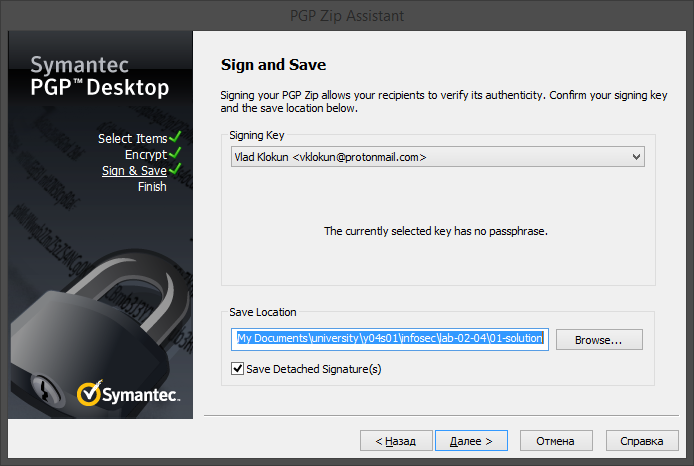
\includegraphics[width = \columnwidth]{./assets/p16.png}
				\caption{}
				\label{subfig:sign}
			\end{subfigure}%
			\hspace{1em}%
			\begin{subfigure}[b]{6 \gridunitwidth - 1em / (2-1)}
				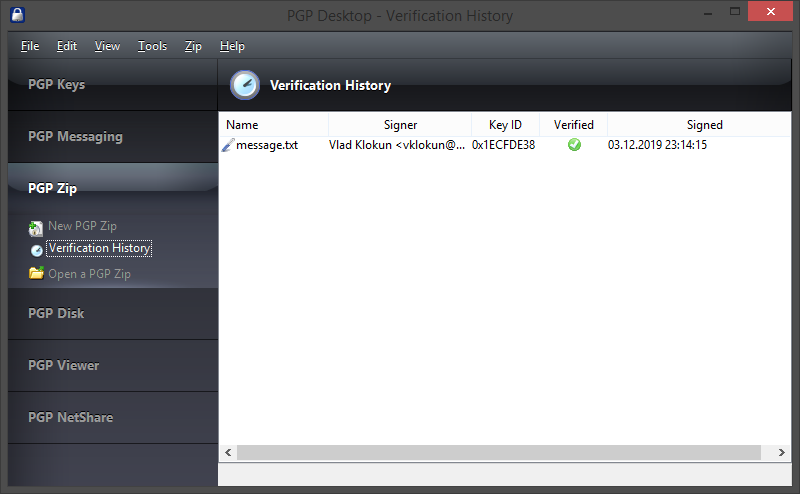
\includegraphics[width = \columnwidth]{./assets/p17.png}
				\caption{}
				\label{subfig:verify}
			\end{subfigure}
			\caption{Результати цифрового підпису та перевірки підписаного файлу}
			\label{fig:sign-verify-file}
		\end{figure}

		Підписуємо публічний ключ іншої людини, знайдений серед ключів, доступних криптографічній системі~(рис.~\ref{fig:sign-verify-key}).

		\begin{figure}[!htbp]
			\centering
			\begin{subfigure}[b]{8 \gridunitwidth - 1em / (2-1)}
				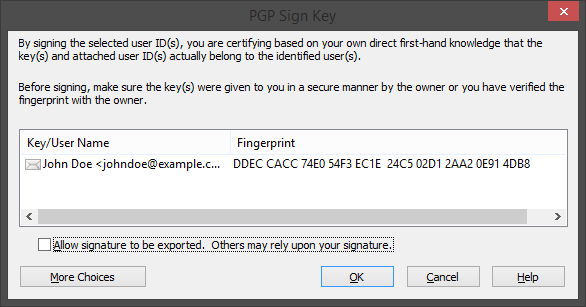
\includegraphics[width = \columnwidth]{./assets/p18.png}
				\caption{}
				\label{subfig:sign-key}
			\end{subfigure}%
			\hspace{1em}%
			\begin{subfigure}[b]{8 \gridunitwidth - 1em / (2-1)}
				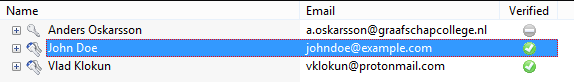
\includegraphics[width = \columnwidth]{./assets/p19.png}
				\caption{}
				\label{subfig:verify-key}
			\end{subfigure}
			\caption{Результати цифрового підпису та перевірки підписаного публічного ключа}
			\label{fig:sign-verify-key}
		\end{figure}

		Додаємо і видаляємо компоненти ключа. Для цього заходимо у властивості створеного ключа і генеруємо новий підключ.

		\begin{figure}[!htbp]
			\centering
			\begin{subfigure}[b]{5 \gridunitwidth - 1em / (2-1)}
				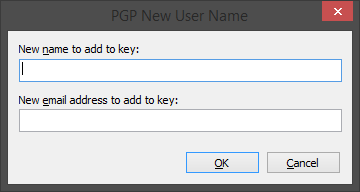
\includegraphics[width = \columnwidth]{./assets/p20.png}
				\caption{}
				\label{subfig:add-subname}
			\end{subfigure}%
			\hspace{1em}%
			\begin{subfigure}[b]{4 \gridunitwidth - 1em / (2-1)}
				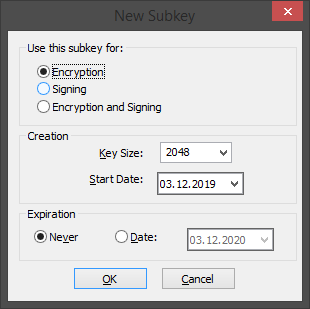
\includegraphics[width = \columnwidth]{./assets/p21.png}
				\caption{}
				\label{subfig:add-subkey}
			\end{subfigure}
			\begin{subfigure}[b]{9 \gridunitwidth - 1em / (2-1)}
				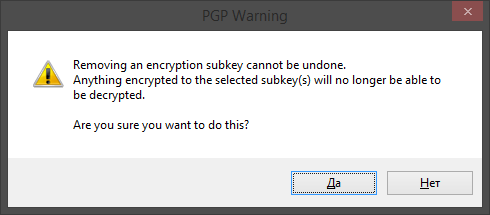
\includegraphics[width = \columnwidth]{./assets/p22.png}
				\caption{}
				\label{subfig:remove-subkey}
			\end{subfigure}
			\caption{Додавання і видалення компонентів ключа}
			\label{fig:add-key-components}
		\end{figure}

		Створюємо відкликаючий сертифікат та відкликаємо ключ з його допомогою~(рис.~\ref{fig:revocation}).

		\begin{figure}[!htbp]
			\centering
			\begin{subfigure}[b]{8 \gridunitwidth - 1em / (2-1)}
				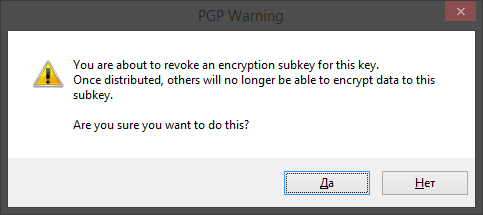
\includegraphics[width = \columnwidth]{./assets/p23.png}
				\caption{}
				\label{subfig:revoke-subkey}
			\end{subfigure}
			\begin{subfigure}[b]{8 \gridunitwidth - 1em / (2-1)}
				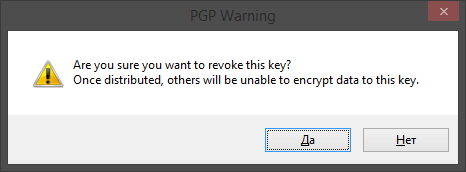
\includegraphics[width = \columnwidth]{./assets/p24.png}
				\caption{}
				\label{subfig:revoke-key}
			\end{subfigure}
			\caption{Додавання і видалення компонентів ключа}
			\label{fig:revocation}
		\end{figure}

		\subsection{Асиметричне шифрування в операційній системі~\textenglish{\allcaps{GNU}/Linux}}
			Для роботи з криптографією з відкритим ключем в операційній системи~\textenglish{\allcaps{GNU}/Linux} будемо використовувати програмну систему~\textenglish{\allcaps{GNU} Privacy Guard}. Генеруємо пару ключів: публічний і приватний~(рис.~\ref{fig:gpg-gen-keys}).

		\begin{figure}[!htbp]
			\centering
			\begin{subfigure}[b]{6 \gridunitwidth - 1em / (2-1)}
				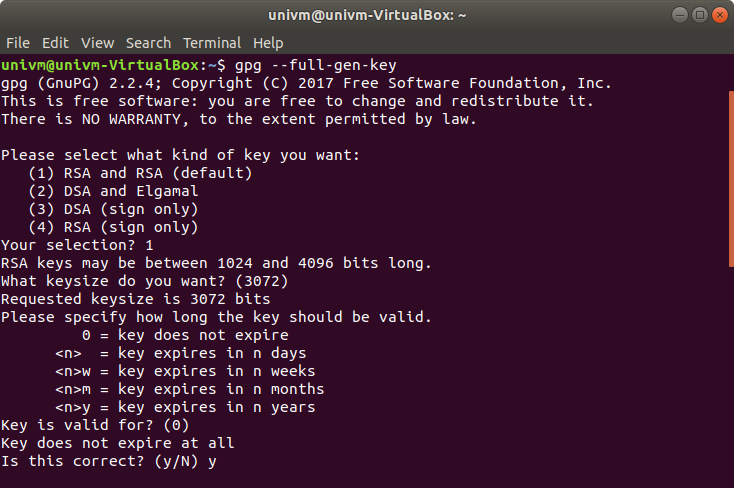
\includegraphics[width = \columnwidth]{./assets/p25.png}
				\caption{}
				\label{subfig:gpg-gen-keys-01}
			\end{subfigure}%
			\hspace{1em}%
			\begin{subfigure}[b]{6 \gridunitwidth - 1em / (2-1)}
				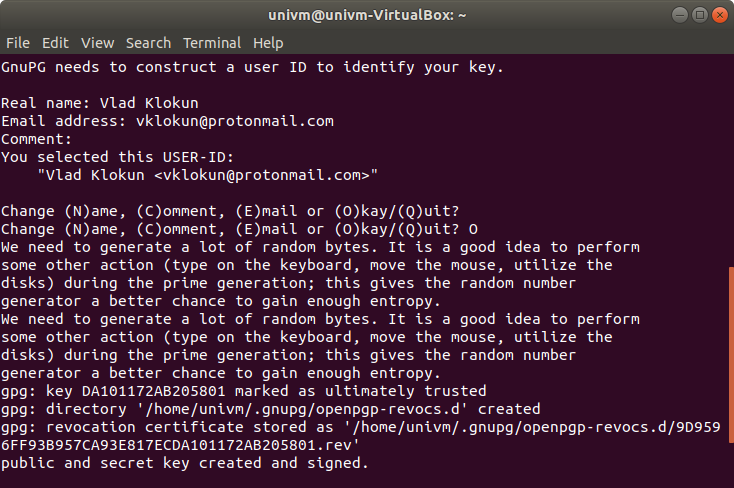
\includegraphics[width = \columnwidth]{./assets/p26.png}
				\caption{}
				\label{subfig:gpg-gen-keys-02}
			\end{subfigure}
			\begin{subfigure}[b]{9 \gridunitwidth - 1em / (2-1)}
				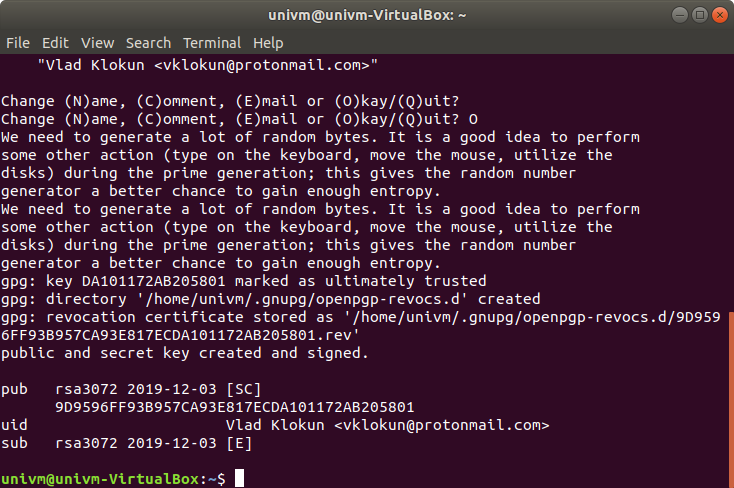
\includegraphics[width = \columnwidth]{./assets/p27.png}
				\caption{}
				\label{subfig:gpg-gen-keys-03}
			\end{subfigure}
			\caption{Генерація публічного і приватного ключа в~\textenglish{\allcaps{GNU} Privacy Guard}}
			\label{fig:gpg-gen-keys}
		\end{figure}

		Експортуємо згенерований ключ і перевіряємо список усіх доступних ключів~(рис.~\ref{fig:gpg-export-list-keys}).

		\begin{figure}[!htbp]
			\centering
			\begin{subfigure}[b]{6 \gridunitwidth - 1em / (2-1)}
				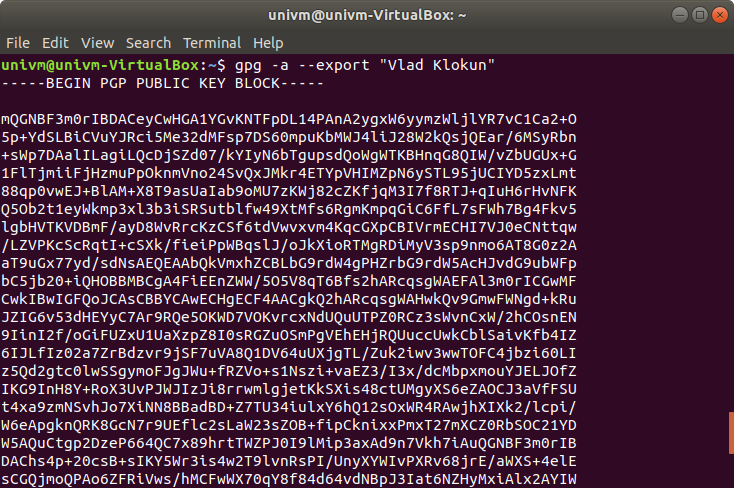
\includegraphics[width = \columnwidth]{./assets/p28.png}
				\caption{}
				\label{subfig:gpg-export-key}
			\end{subfigure}%
			\hspace{1em}%
			\begin{subfigure}[b]{6 \gridunitwidth - 1em / (2-1)}
				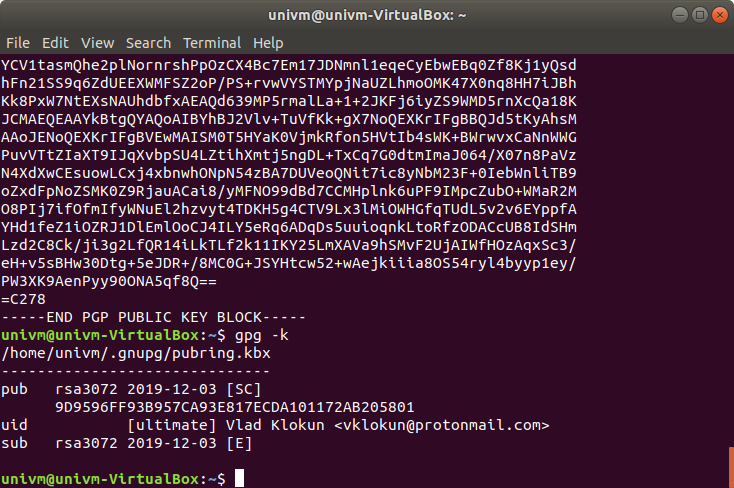
\includegraphics[width = \columnwidth]{./assets/p29.png}
				\caption{}
				\label{subfig:gpg-list-keys}
			\end{subfigure}
			\caption{Експорт згенерованого ключа і перевірка списку доступних ключів в~\textenglish{\allcaps{GNU} Privacy Guard}}
			\label{fig:gpg-export-list-keys}
		\end{figure}

		Знаходимо ключ іншої людини, імпортуємо та перевіряємо його цілісність~(рис.~\ref{fig:gpg-import-key}).

		\begin{figure}[!htbp]
			\centering
			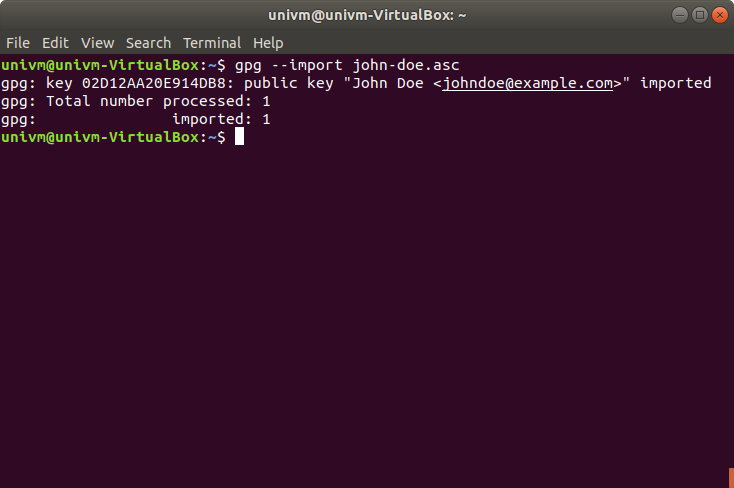
\includegraphics[width = \columnwidth]{./assets/p30.png}
			\caption{Імпорт і перевірка ключа іншої людини в~\textenglish{\allcaps{GNU} Privacy Guard}}
			\label{fig:gpg-import-key}
		\end{figure}

		Шифруємо та дешифруємо просте повідомлення за допомогою публічного ключа. Потім підписуємо повідомлення і перевіряємо його цілісність~(рис.~\ref{fig:gpg-enc-dec-sign-verify}).

		\begin{figure}[!htbp]
			\centering
			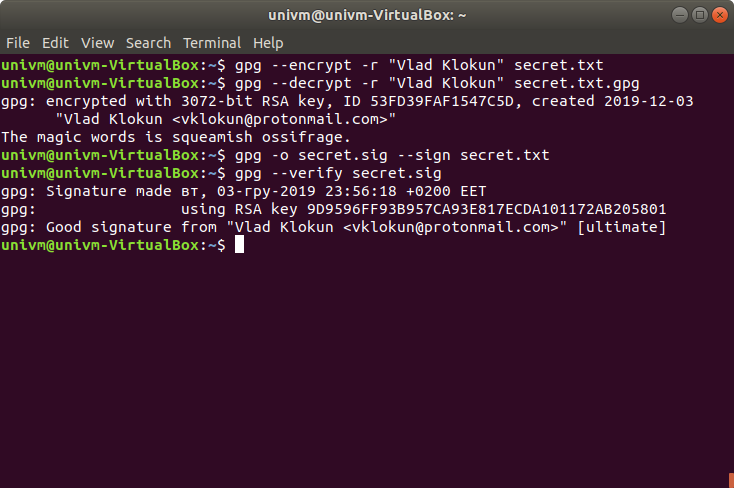
\includegraphics[width = \columnwidth]{./assets/p31.png}
			\caption{Шифрування, розшифрування, підпис і перевірка цілісності повідомлення в~\textenglish{\allcaps{GNU} Privacy Guard}}
			\label{fig:gpg-enc-dec-sign-verify}
		\end{figure}

		Отже, на цьому робота з криптографічною системою з відкритим ключем завершена.
		\section{Висновок}
			Виконуючи дану лабораторну роботу, ми ознайомилися з~основними поняттями асиметричних криптографічних систем і встановили програмне забезпечення для ОС Windows та GNU/Linux, що виконує криптографічні операції з відкритим ключем, та навчилися його використовувати.
\end{document}
